% \documentclass[handout, xcolor=table]{beamer}
\documentclass[xcolor=table]{beamer}

%-----------------------[ Macros ]----------------------------------------------%

%-----------------------[ Packages ]-------------------------------------------%

\usepackage[utf8]{inputenc}
\usepackage[brazilian]{babel}
% \usepackage[english]{babel}
\usepackage[T1]{fontenc}
\usepackage{lmodern}
\usepackage{amsfonts}
\usepackage{indentfirst}
\usepackage{xspace}
\usepackage{setspace}
\usepackage{geometry}
\usepackage{mathtools}
\usepackage{amsmath}
\usepackage{amsthm}
\usepackage{subcaption}
\usepackage{pdfpages}
\usepackage{hanging}
\usepackage{pdfpages}
\usepackage{nicefrac}
\usepackage{graphicx}
\usepackage[labelformat=empty]{caption}
\usepackage{booktabs, multirow} % for borders and merged ranges
\usepackage[hyperpageref]{backref}
% \usepackage[
%   scr=boondox, % heavily sloped
%   cal=esstix % slightly sloped
% ]{mathalpha}
\usepackage{xmpmulti}
\usepackage{appendixnumberbeamer}

% Tikz:
\usepackage{tikz}
% \usetikzlibrary{ipe} % ipe compatibility library
\usetikzlibrary{calc, arrows, arrows.meta, patterns}

%-----------------------[ Colors ]---------------------------------------------%

\definecolor{red}{rgb}{1,0,0}
\definecolor{blue}{rgb}{0,0,1}
\definecolor{green}{rgb}{0,1,0}
\definecolor{yellow}{rgb}{1,1,0}
\definecolor{orange}{rgb}{1,0.647,0}
\definecolor{gold}{rgb}{1,0.843,0}
\definecolor{purple}{rgb}{0.627,0.125,0.941}
\definecolor{gray}{rgb}{0.745,0.745,0.745}
\definecolor{brown}{rgb}{0.647,0.165,0.165}
\definecolor{navy}{rgb}{0,0,0.502}
\definecolor{pink}{rgb}{1,0.753,0.796}
\definecolor{seagreen}{rgb}{0.18,0.545,0.341}
\definecolor{turquoise}{rgb}{0.251,0.878,0.816}
\definecolor{violet}{rgb}{0.933,0.51,0.933}
\definecolor{darkblue}{rgb}{0,0,0.545}
\definecolor{darkcyan}{rgb}{0,0.545,0.545}
\definecolor{darkgray}{rgb}{0.663,0.663,0.663}
\definecolor{darkgreen}{rgb}{0,0.392,0}
\definecolor{darkmagenta}{rgb}{0.545,0,0.545}
\definecolor{darkorange}{rgb}{1,0.549,0}
\definecolor{darkred}{rgb}{0.545,0,0}
\definecolor{lightblue}{rgb}{0.678,0.847,0.902}
\definecolor{lightcyan}{rgb}{0.878,1,1}
\definecolor{lightgray}{rgb}{0.827,0.827,0.827}
\definecolor{lightgreen}{rgb}{0.565,0.933,0.565}
\definecolor{lightyellow}{rgb}{1,1,0.878}
\definecolor{black}{rgb}{0,0,0}
\definecolor{white}{rgb}{1,1,1}

%-----------------------[ Commands ]-------------------------------------------%

\newcommand\mycomment[1]{} % block comment

\newcommand{\FPT}{\ensuremath{\mathcal{F}\mathcal{P}\mathcal{T}}\xspace}
\newcommand{\XP}{\ensuremath{\mathsf{XP}}\xspace}
\newcommand{\PP}{\ensuremath{\mathrm{P}}\xspace}
\newcommand{\NP}{\ensuremath{\mathrm{NP}}\xspace}

\newcommand{\dist}{\text{dist}}
\newcommand{\cost}{\text{cost}}
\newcommand{\opt}{\text{OPT}}
\newcommand{\makespan}{\emph{makespan}}

\newcommand{\cala}{\mathcal{A}}
\newcommand{\calb}{\mathcal{B}}
\newcommand{\cali}{\mathcal{I}}
\newcommand{\call}{\mathcal{L}}
\newcommand{\calo}{\mathcal{O}}
\newcommand{\cals}{\mathcal{S}}
\newcommand{\calt}{\mathcal{T}}

\newcommand{\R}{\rm I\!R}
\newcommand{\N}{\rm I\!N}
\newcommand{\overeps}{\nicefrac{1}{\varepsilon}}
\newcommand{\B}{$\bullet$}

\newcommand\rest[2]{\left.{#1}\right|_{#2}} % function restriction

\DeclarePairedDelimiter\ceil{\lceil}{\rceil}
\DeclarePairedDelimiter\floor{\lfloor}{\rfloor}
\DeclareMathOperator*{\argmax}{arg\,max}
\DeclareMathOperator*{\argmin}{arg\,min}

%-----------------------[ Proof Environments ]---------------------------------%

% \newtheorem{definition}{Definição}
\newtheorem{thm}{Teorema}
\newtheorem{cor}{Corolário}
\newtheorem{conj}{Conjectura}
\newtheorem{lem}{Lema}
\newtheorem{obs}{Observação}


\newcounter{finalframe}
\newcommand{\stopcounter}{
  \setcounter{finalframe}{\insertframenumber}
}

\newcommand{\resumecounter}{
  \setcounter{framenumber}{\value{finalframe}}
}

\newcommand{\inccounter}{
  \setcounter{framenumber}{\value{finalframe} + 1}
}

%-----------------------[ Template ]-------------------------------------------%

\mode<presentation> {
    \usetheme[sectionpage=none, progressbar=frametitle, block=fill]{moloch} % modern fork of the metropolis theme
    \setbeamertemplate{footline}[frame number] % to replace the footer line in all slides with a simple slide count
}
\setbeamerfont{footnote}{size=\tiny}
\setbeamertemplate{navigation symbols}{}
\setbeamertemplate{footnote}{%
    \hangpara{2em}{1}%
    \makebox[2em][l]{\tiny\insertfootnotemark}%
    \hspace{-1em}\tiny\insertfootnotetext\par\vspace{0.2cm}%
}

%-----------------------[ (Sub)Section Slides ]--------------------------------%

% \AtBeginSection[]{
%     \begin{frame}
%     \vfill
%     \centering
%     \begin{beamercolorbox}[sep=8pt,center,shadow=true]{title}
%         \usebeamerfont{title}\insertsectionhead\par%
%     \end{beamercolorbox}
%     \vfill
%     \end{frame}
% }

\makeatletter
\newcommand{\subseqslide}{
\begin{frame}
    \setbeamercolor{title}{bg=mDarkTeal,fg=black!2}
  \centering
  \begin{minipage}{22em}
    \raggedright
    \begin{beamercolorbox}[sep=8pt,center,shadow=true]{title}
        \usebeamerfont{title}\insertsectionhead\par%
    \end{beamercolorbox}
    \usebeamertemplate*{progress bar in section page}
    \par
    \ifx\insertsubsectionhead\@empty\else%
      \vskip-.6\baselineskip
      \usebeamercolor[fg]{subsection title}%
      \usebeamerfont{subsection title}%
      \insertsubsectionhead{}
    \fi
  \end{minipage}
  \par
  \vspace{\baselineskip}
\end{frame}
}

\AtBeginSubsection[]{%
\subseqslide

\setcounter{tocdepth}{3}
\frame<beamer>{ 
  \frametitle{}
  \centering
  \begin{minipage}{20em}
  \tableofcontents[
    currentsection,currentsubsection,sectionstyle=show/hide,subsectionstyle=show/shaded/hide,subsubsectionstyle=show/show/hide/hide
  ]    
  \end{minipage}
  
}
}
\makeatother

\makeatletter
\AtBeginSubsubsection[]{%
\begin{frame}
  \centering
  \begin{minipage}{22em}
    \raggedright
    \usebeamercolor[fg]{section title}
    \usebeamerfont{section title}
    \insertsubsectionhead{}\\[-1ex]
    \usebeamertemplate*{progress bar in section page}
    \par
    \ifx\insertsubsectionhead\@empty\else%
      \vskip-.6\baselineskip
      \usebeamercolor[fg]{subsection title}%
      \usebeamerfont{subsection title}%
      \insertsubsubsectionhead
    \fi
  \end{minipage}
  \par
  \vspace{\baselineskip}
\end{frame}
}
\makeatother

%-----------------------[ Title page ]-----------------------------------------%

\title{
  Algoritmos para o Freeze-Tag e Problemas de Robótica de Enxame Relacionados%
  \texorpdfstring{\footnote{Financiado pela Fundação de Amparo à Pesquisa do
  Estado de São Paulo~(FAPESP) processo \mbox{\#2022/13435-4}}}{}
}

\titlegraphic{
  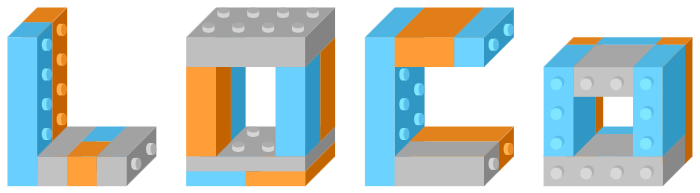
\includegraphics[height=0.8cm]{logos/loco.png}
  \hspace{4.25cm}
  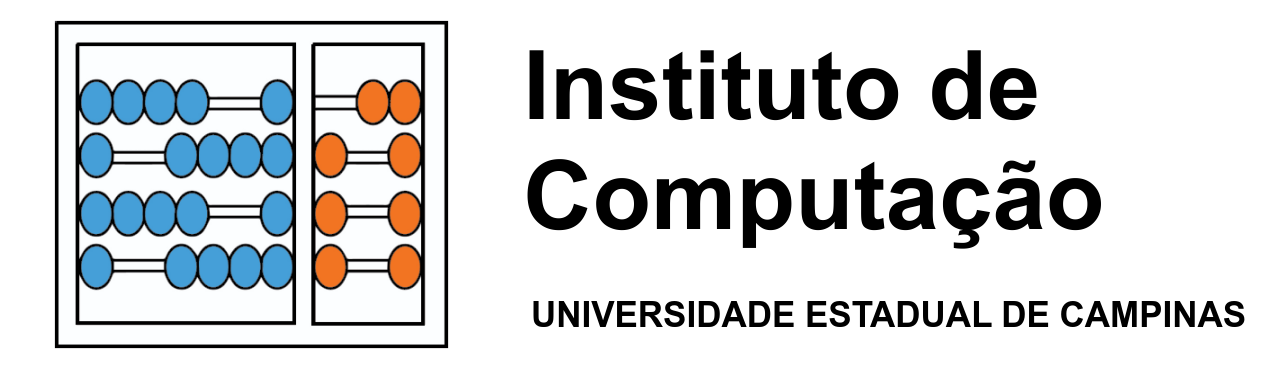
\includegraphics[height=1cm]{logos/ic.png}
}

\author{
  Aluno: Lucas de Oliveira Silva\texorpdfstring{\\}{}
  Orientador: Lehilton Lelis Chaves Pedrosa
}

\institute{Instituto de Computação, Unicamp}

\date{10 de Março de 2025}

\begin{document}

\begin{frame}[plain]
  \titlepage
\end{frame}

\setcounter{tocdepth}{1}
\begin{frame}{Sumário}
  \tableofcontents
\end{frame}

%------------------------------------------------------------------------------%

\section{Problemas Estudados}

\subsection{Freeze-Tag Problem}
%------------------------------------------------------------------------------%

\subsubsection{Contexto}

\stopcounter
\begin{frame}{Origem}
  O Freeze-Tag Problem (FTP) surge como um problema de robótica de enxame em 2002~\cite{Arkin02}:
  \bigbreak
  \begin{minipage}{\linewidth}
    \centering
    \multiinclude[format=png, start=0, end=5, graphics={height=5cm}]{FTP/ftp_example/Temp}
  \end{minipage}
\end{frame}
\inccounter

\begin{frame}{Motivação}
  \begin{itemize}[<+->]

    \item Modela problemas de transmissão de dados e design de redes;

    \item Soluções são árvores binárias geradoras de altura mínima;

    \item Ligado às árvores de multicast (estruturas de comunicação da camada de aplicação).

  \end{itemize}
\end{frame}

\begin{frame}{Definição - Instância}
  \begin{itemize}[<+->]

    \item Conjunto de $n$ robôs $R$;

    \item Robô inicial $r_0 \in R$ (\textbf{fonte});

    \item Função de distância $\dist\colon R\times R \to \R^+$.

  \end{itemize}
\end{frame}

\stopcounter
\begin{frame}{Definição - Solução}
  O conjunto de movimentos (\textbf{\emph{schedule}} ou \textbf{árvore de ativação}):

  \pause

  \begin{itemize}[<+->]
    \item Árvore binária $\calt$ enraizada em $r_0$ que visita todos os robôs;

    \item Minimizamos o \textbf{\emph{makespan}}, isto é, o tempo total de ativação.
  \end{itemize}

  \pause
  \bigskip
  \begin{minipage}{\linewidth}
    \centering
    \multiinclude[format=png, start=0, end=5, graphics={height=5cm}]{FTP/solution/Temp}
  \end{minipage}
\end{frame}
\inccounter

%------------------------------------------------------------------------------%

\subsubsection{Resultados Teóricos}

\begin{frame}{Resultado Anterior}
  \begin{thm}[Arkin et al.~\cite{Arkin02}]
    O FTP é fortemente NP-difícil em estrelas com pesos nas arestas.
  \end{thm}
\end{frame}

\begin{frame}{Nossos Resultados}
  \setbeamercolor{block body}{bg=green!35!white}
  \begin{cor}[Pedrosa e Silva~\cite{Pe23}]
    O FTP é NP-difícil em árvores binárias enraizadas, sem pesos nas arestas, com a fonte na raiz e robôs desativados apenas nas folhas.
  \end{cor}

  \pause
  \begin{cor}[Pedrosa e Silva~\cite{Pe23}]
    O FTP é fortemente NP-difícil em árvores ternárias enraizadas, com pesos nas arestas, a fonte na raiz e um robô desativado em cada outro nó.
  \end{cor}
\end{frame}

\begin{frame}{Resultado Anterior}
  \begin{thm}[Arkin et al.~\cite{Arkin02}]
    É NP-difícil aproximar o FTP em grafos com pesos nas arestas dentro de um fator menor que $\nicefrac{5}{3}$, mesmo se o grafo tiver grau máximo $4$ e possuir exatamente um robô em cada nó.
  \end{thm}
\end{frame}

\begin{frame}{Nosso Resultado}
  \setbeamercolor{block body}{bg=green!35!white}
  \begin{thm}
    É NP-difícil aproximar o FTP em grafos sem pesos nas arestas dentro de um fator de até $\nicefrac{3}{2}$, mesmo se o grafo tiver diâmetro $2$ e possuir ao menos um robô em cada nó.
  \end{thm}
\end{frame}

\begin{frame}{Conjectura Inicial}
  \begin{conj}[Arkin et al.~\cite{Arkin06}]
    O FTP é NP-difícil para as distâncias Euclidiana ($L_2$) ou de Manhattan ($L_1$) no plano $\R^2$.
  \end{conj}

  \pause
  Problema 35 do \emph{The Open Problems Project}~\cite{TOPP}.
\end{frame}

\begin{frame}{Resultados Anteriores}
  \begin{thm}[Arkin et al.~\cite{Arkin02}]
    Existe um EPTAS para o FTP com distâncias $L_p$ em qualquer espaço de dimensão fixa $\R^d$, com tempo de execução $O(n \log n) + 2^{O((\overeps)^2\log{\overeps})}$.
  \end{thm}

  \pause
  \begin{thm}[Abel et al.~\cite{Yu17}]
    O FTP é NP-difícil para distância $L_2$ no plano.
  \end{thm}

  \pause
  \begin{thm}[Demaine e Rudoy~\cite{Erik17}]
    O FTP é NP-difícil para distâncias $L_p$, onde $p>1$, em 3D.
  \end{thm}
\end{frame}

\begin{frame}{Nossos Resultados}
  \setbeamercolor{block body}{bg=green!35!white}
  \begin{thm}[Pedrosa e Silva~\cite{Lu23}]
    O FTP é fortemente NP-difícil para distância $L_1$ em 3D.
  \end{thm}

  \pause
  \begin{cor}[Pedrosa e Silva~\cite{Lu23}]
    O FTP é NP-difícil em grades 3D sem pesos nas arestas.
  \end{cor}
\end{frame}

%------------------------------------------------------------------------------%

\subsubsection{Resultados Experimentais}

\begin{frame}{Abordagens Exatas}
  \begin{itemize}[<+->]

    \item Experimentos foram realizados devido à ausência de implementações exatas;

    \item Duas formulações MIP implementadas usando Gurobi;

    \item Uma formulação CP implementada usando o CP-SAT do Google OR-Tools;

    \item Avaliação feita com instâncias usando a distância $L_2$ em $\R^2$.

  \end{itemize}
\end{frame}

\begin{frame}{Tornando um PTAS mais Prático}
  Implementamos o EPTAS de Arkin et al.~\cite{Arkin06}, substituindo a enumeração lenta do algoritmo por nossa formulação CP.

  \bigskip
  \begin{minipage}{\linewidth}
    \centering
    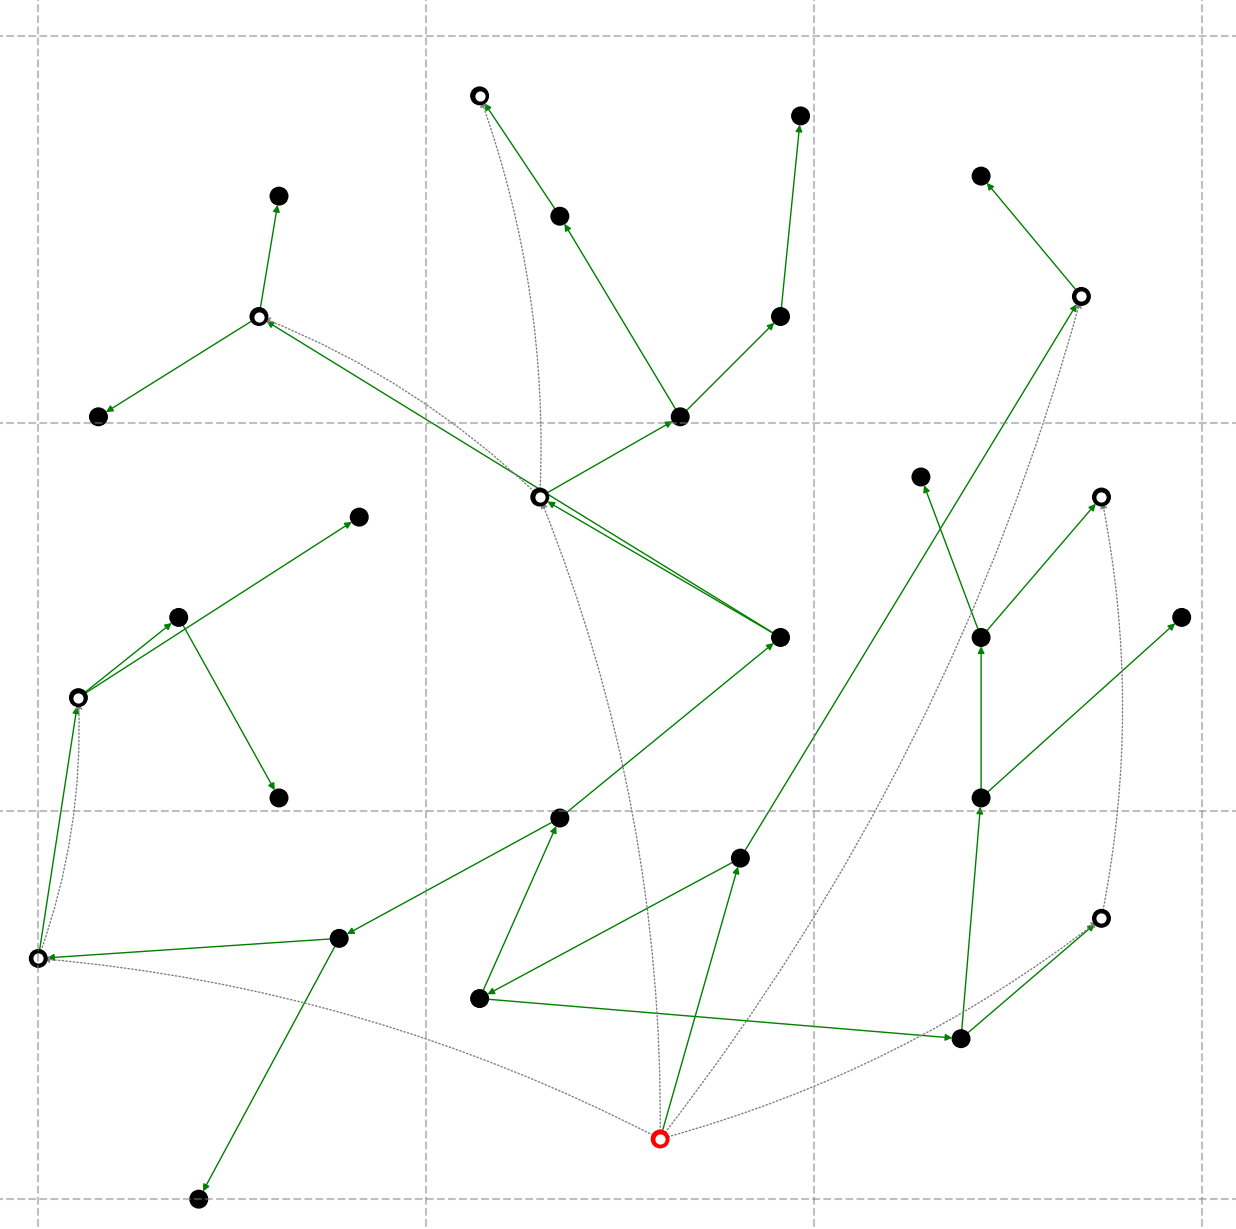
\includegraphics[height=6.7cm]{FTP/ptas_solver.png}
  \end{minipage}
\end{frame}


\subsection{Angular Freeze-Tag Problem}
%------------------------------------------------------------------------------%

\subsubsection{Contexto}

\stopcounter
\begin{frame}{Origem}
  O \textbf{Angular Freeze-Tag Problem} (AFTP) surge como um problema de \textbf{\emph{broadcast}} entre satélites em 2018~\cite{Fe18}:
  \bigbreak
  \begin{minipage}{\linewidth}
    \centering
    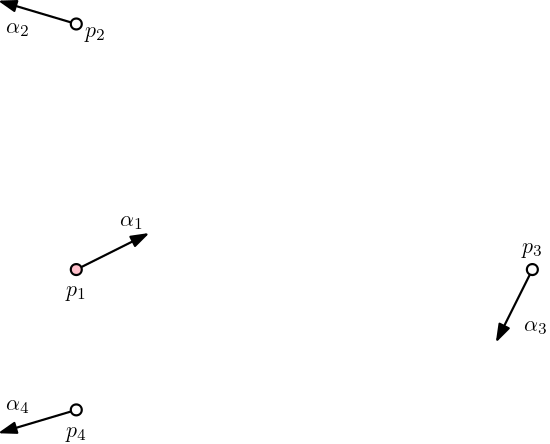
\includegraphics[height=4cm]{AFTP/instance/Temp-0.png}
  \end{minipage}
\end{frame}
\inccounter

\begin{frame}{Motivação}
  \begin{itemize}[<+->]

    \item Recursos limitados restringem o movimento dos satélites;

    \item Grandes distâncias impossibilitam um \emph{broadcast} simultâneo;

    \item O crescimento das constelações de satélites.

  \end{itemize}
\end{frame}

\begin{frame}{Definição - Instância}
  \begin{itemize}[<+->]

    \item Conjunto $P = \{p_1, \dots, p_n\}\subseteq \R^d$ de posições distintas;

    \item Cada $p_i$ corresponde a um satélite associado a $\alpha_i$;

    \item Inicialmente, apenas $p_1$ contém um dado a ser propagado.

  \end{itemize}
\end{frame}

\begin{frame}{Definição - Solução}
  As sequências de rotações onde o objetivo é minimizar o \emph{makespan}:

  \pause

  \bigskip
  \begin{minipage}{\linewidth}
    \centering
    \colorbox{white}{\multiinclude[format=png, start=0, end=3, graphics={height=5.5cm}]{AFTP/instance/Temp}}
  \end{minipage}
\end{frame}

%------------------------------------------------------------------------------%

\subsubsection{Resultados Anteriores e Novos}

\begin{frame}{Resultados Anteriores}
  \begin{thm}[Fekete e Krupke~\cite{Fe18}]
    É NP-difícil aproximar o AFTP em 2D dentro de um fator menor que $\nicefrac{5}{3}$.
  \end{thm}

  \pause

  \begin{thm}[Fekete e Krupke~\cite{Fe18}]
    Existe uma $9$-aproximação para o AFTP em 2D, assumindo um limite inferior de $\varepsilon>0$ para a rotação inicial de qualquer satélite que rotacione sua antena.
  \end{thm}
\end{frame}

\begin{frame}{Nossos Resultados}
  \setbeamercolor{block body}{bg=green!35!white}
  Chamamos de \textbf{energia total} de uma solução a soma da rotação total realizada por todos os satélites.

  \pause

  \begin{thm}
    Seja $I$ uma instância do AFTP em 2D, $\mathbf{F}$ um número real e $\mathbf{k}$ um inteiro positivo.
    %
    Então, existe um algoritmo que roda em tempo ${(n\frac{Fk}{\varepsilon})^{O(\frac{Fk}{\varepsilon})}}$ e ou prova que toda solução ótima requer mais de $F$ de energia total, ou encontra uma solução com \emph{makespan} no máximo ${(1+\nicefrac{1}{k})\opt(I)}$.
  \end{thm}

  \pause

  \begin{thm}
    Para todo inteiro positivo $k$, existe uma \mbox{$(1+\nicefrac{1}{k})$-aproximação} para o AFTP em 2D com o objetivo de minimizar a energia total, que roda em tempo \mbox{$(n\frac{k}{\varepsilon})^{O(\frac{k}{\varepsilon})}$}.
  \end{thm}
\end{frame}


\subsection{Minimum Scan Cover}
%------------------------------------------------------------------------------%

\subsubsection{Contexto}

\begin{frame}{Origem}
  O Minimum Scan Cover (MSC) foi introduzido em 2021~\cite{Fe21} como um problema de comunicação ponto a ponto entre satélites:
  \bigbreak
  \begin{minipage}{\linewidth}
    \centering
    \only<1>{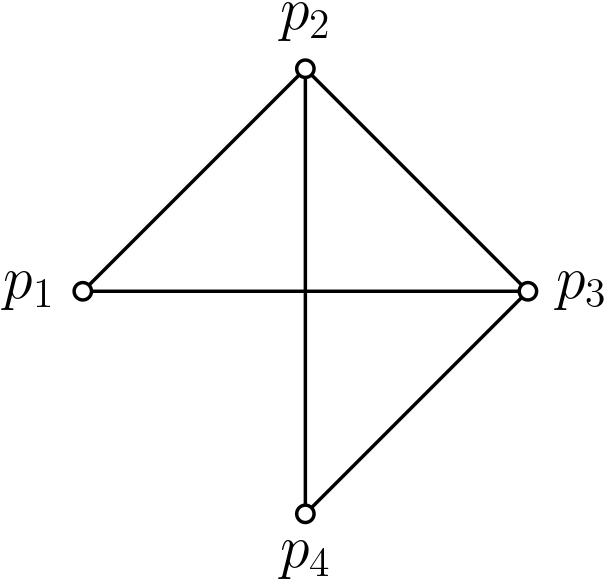
\includegraphics[height=5cm]{MSC/instance/Temp-0.png}}%
    \only<2>{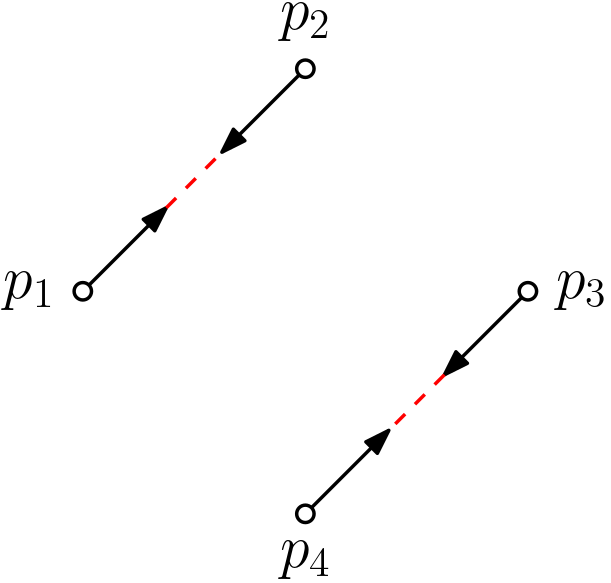
\includegraphics[height=5cm]{MSC/instance/Temp-1.png}}%
    \only<3>{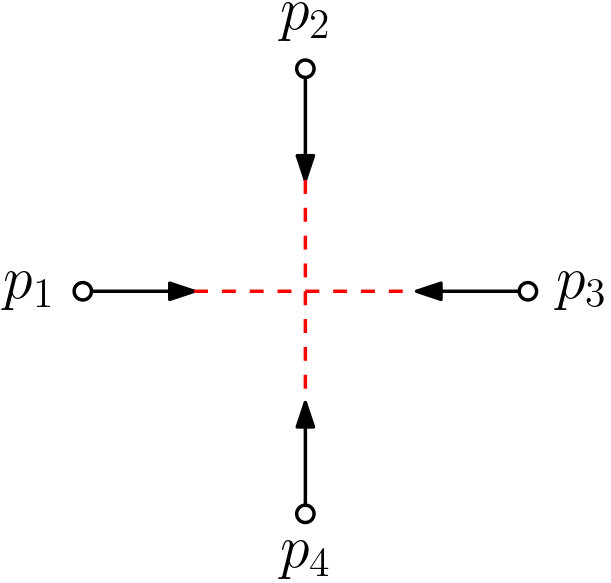
\includegraphics[height=5cm]{MSC/instance/Temp-2.png}}%
    \only<4>{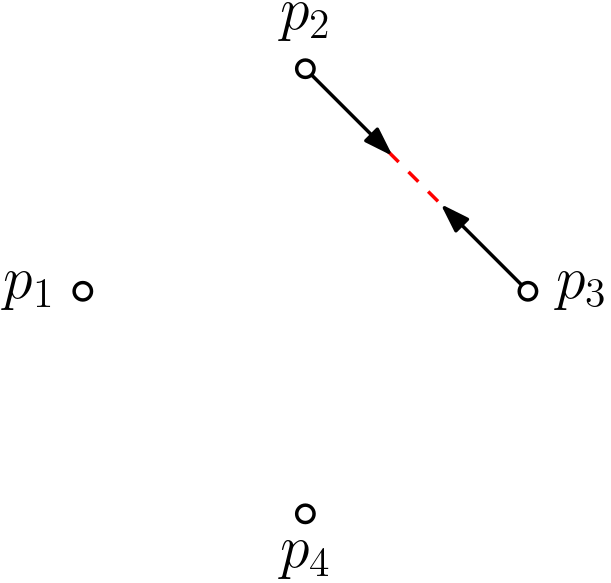
\includegraphics[height=5cm]{MSC/instance/Temp-3.png}}%
  \end{minipage}
\end{frame}

\begin{frame}{Motivação}
  \begin{itemize}[<+->]

    \item É possível usar tanto transmissão direcional quanto recepção omnidirecional;

    \item Mas exige duas antenas, aumentando custo e complexidade.

  \end{itemize}
\end{frame}

\begin{frame}{Definição - Instância}
  \begin{itemize}[<+->]

    \item Conjunto $P = \{p_1, \dots, p_n\}\subseteq \R^d$ de posições distintas;

    \item Grafo $G=(P, E)$ onde $E\subseteq P\times P$.

  \end{itemize}
\end{frame}

\begin{frame}{Definição - Solução}
  \textbf{Escalonamento} ${\cals\colon E\to \R^+}$ onde queremos minimizar $\max\limits_{e \in E} \cals(e)$:
  \begin{minipage}{\linewidth}
    \centering
    \vspace*{1cm}
    \only<1>{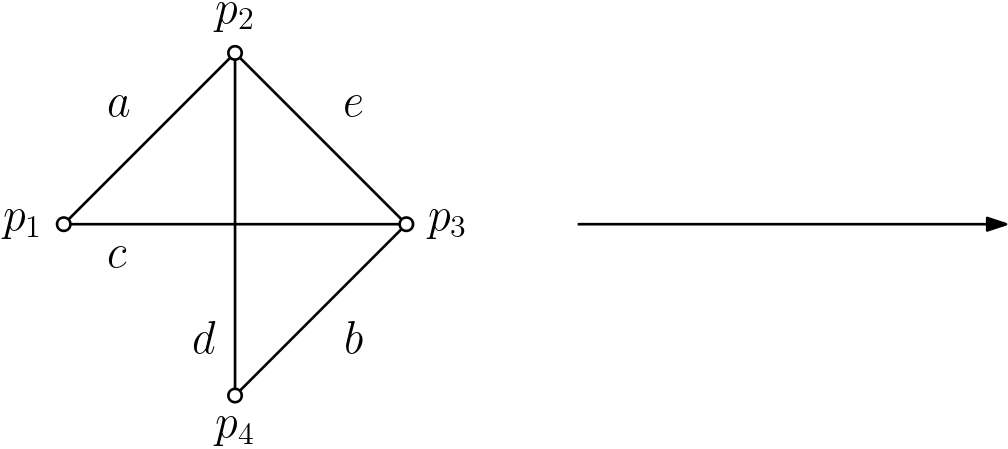
\includegraphics[height=4cm]{MSC/solution/Sol-0.png}}%
    \only<2>{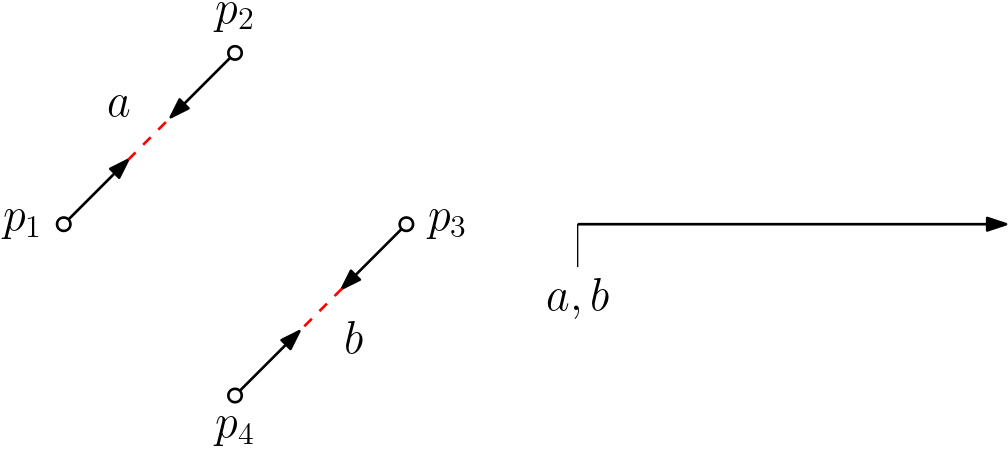
\includegraphics[height=4cm]{MSC/solution/Sol-1.png}}%
    \only<3>{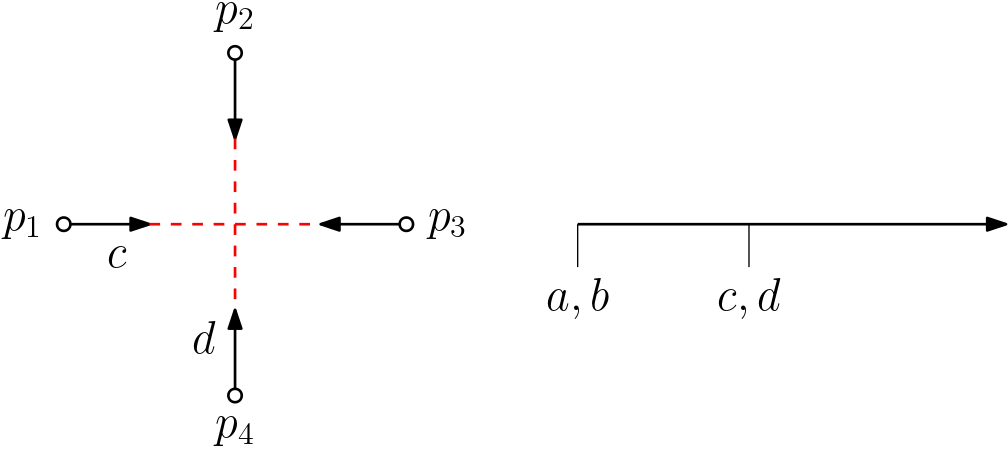
\includegraphics[height=4cm]{MSC/solution/Sol-2.png}}%
    \only<4>{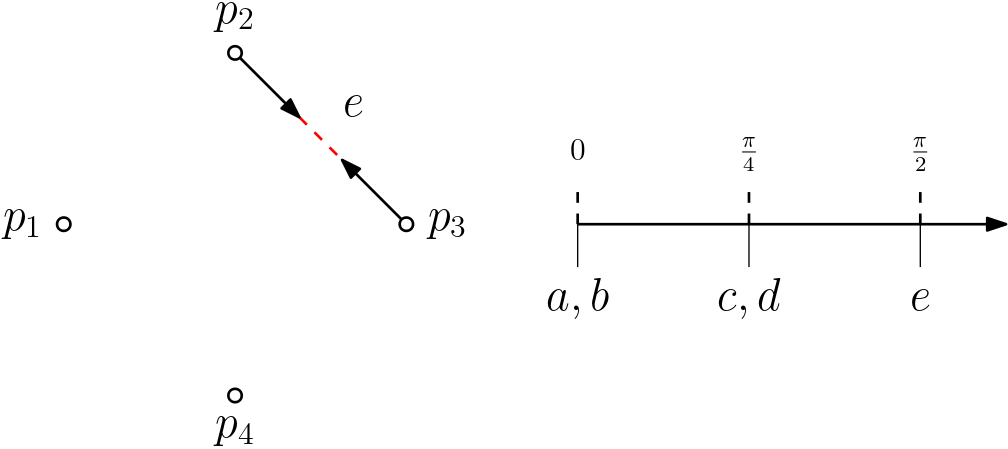
\includegraphics[height=4cm]{MSC/solution/Sol-3.png}\bigbreak}
    \only<4>{$\cals(a)=\cals(b)=0$, $\cals(c)=\cals(d)=\frac{\pi}{4}$ e $\cals(e)=\frac{\pi}{2}$}
  \end{minipage}
\end{frame}

%------------------------------------------------------------------------------%

\subsubsection{Resultados para 1D}

\begin{frame}{Resultado Anterior}
  \begin{thm}[Fekete et al.~\cite{Fe21}]
    Mesmo em 1D, para todo $\gamma \geq 1$, uma $\gamma$-aproximação para o MSC implica que $P = NP$.
  \end{thm}
\end{frame}

\begin{frame}{Nossos Resultados}
  \setbeamercolor{block body}{bg=green!35!white}
  \begin{thm}
    Existe um algoritmo \FPT para o MSC em 1D, parametrizado pela largura de árvore $k$, que roda em tempo $k^{O(k)} \cdot n$.
  \end{thm}

  \pause
  \begin{cor}
    Existe uma $3$-aproximação para o MSC em 1D em grafos planares, que roda em tempo $O(n^2)$.
  \end{cor}
\end{frame}

%------------------------------------------------------------------------------%

\subsubsection{Resultados para 2D}

\begin{frame}{Resultados Anteriores}
  \begin{thm}[Fekete et al.~\cite{Fe21}]
    Mesmo em 2D, para todo $\gamma < \nicefrac{3}{2}$, uma $\gamma$-aproximação para o MSC em grafos bipartidos implica que $P = NP$.
  \end{thm}

  \pause
  \begin{thm}[Fekete et al.~\cite{Fe21}]
    Existe uma $\frac{9}{2}$-aproximação para o MSC em 2D em grafos bipartidos.
  \end{thm}
\end{frame}

\begin{frame}{Preliminares}
  \centering
  Uma instância usando $\ell=8$ direções:

  \bigskip
  \begin{minipage}{\linewidth}
    \centering
    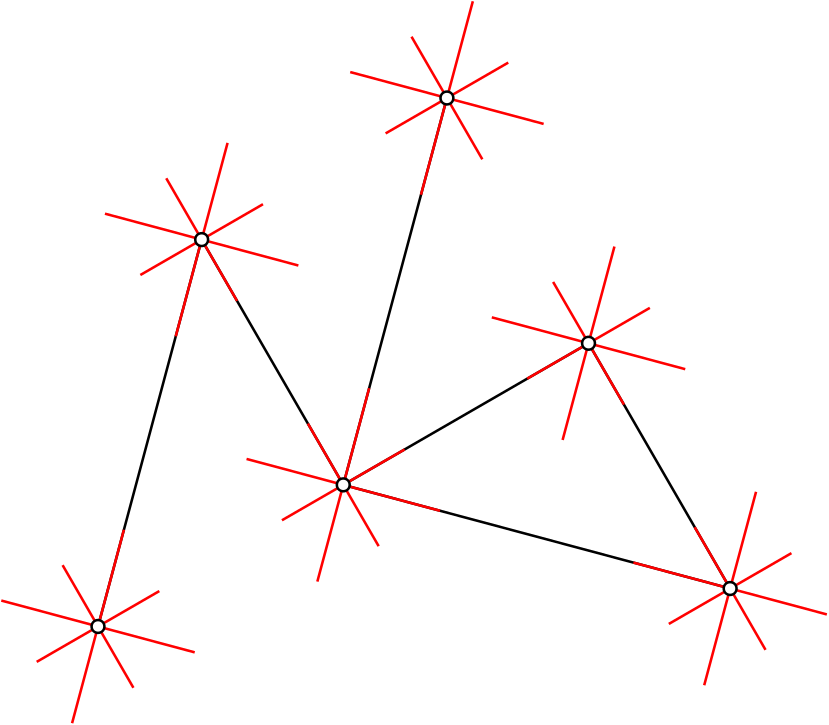
\includegraphics[height=5cm]{MSC/directions.png}
  \end{minipage}
\end{frame}

\begin{frame}{Nossos Resultados}
  \setbeamercolor{block body}{bg=green!35!white}
  \begin{thm}
    Existe um algoritmo \FPT para MSC em 2D, parametrizado pela largura de árvore $k$ e $\ell$, que roda em tempo $k^{O(k \ell \log(\ell))} \cdot n$.
  \end{thm}

  \pause
  \begin{cor}
    Existe uma $3$-aproximação para MSC em 2D em grafos planares parametrizada por $\ell$, que roda em tempo $\ell^{O(\ell)} \cdot n + O(n^2)$.
  \end{cor}
\end{frame}

\begin{frame}{Preliminares}
  \centering
  Uma instância de ângulo mínimo não nulo $\lambda$:

  \bigskip
  \begin{minipage}{\linewidth}
    \centering
    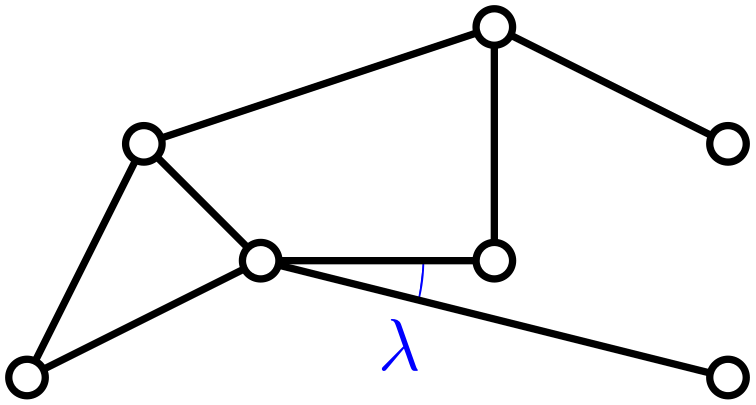
\includegraphics[height=2.5cm]{MSC/lambda.png}
  \end{minipage}
\end{frame}

\begin{frame}{Nosso Resultado}
  \setbeamercolor{block body}{bg=green!35!white}
  \begin{thm}
    Existe uma $2$-aproximação para o MSC em 2D parametrizada pela largura de árvore $k$ e $\lceil \nicefrac{1}{\lambda} \rceil$, que roda em tempo $\lambda^{-O(k^2 + \frac{k \log k}{\lambda})} \cdot (\log k)^{O(k^2)} \cdot n$.
  \end{thm}
\end{frame}

\begin{frame}{Rascunho da Prova}
    \begin{itemize}[<+->]
        \item Seja $\cali = (P, G)$ uma instância de ângulo mínimo não nulo $\lambda$;

        \item Recebemos uma decomposição em árvore de $G$ com largura $k$;

        \item \emph{WLOG}, considere que $\lambda < \pi$.
    \end{itemize}
\end{frame}

\begin{frame}{}
    \begin{itemize}[<+->]
        \item Seja $M := \floor{\nicefrac{\pi}{\lambda}} \geq 1$;

        \item O disco ao redor de cada $p_i\in P$ é dividido em $4M$ \textbf{setores}:
    \end{itemize}
    
    \bigskip
    \pause
    \begin{minipage}{\linewidth}
        \centering
        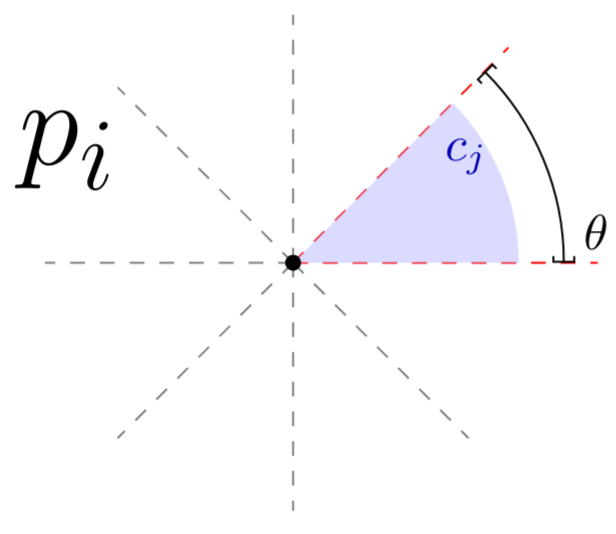
\includegraphics[height=4cm]{MSC/angle.png}
    \end{minipage}

    \bigskip
    \centering
    $\theta := \frac{\pi}{2M} < \lambda$ e os setores são $c_j$ para $j \in [4M-1]$
\end{frame}

\begin{frame}{}
    Consideramos uma relaxação ${\hat \cali:= \cali}$ dependendo de $\theta$:
    
    \bigskip
    \pause
    \begin{minipage}{\linewidth}
        \centering
        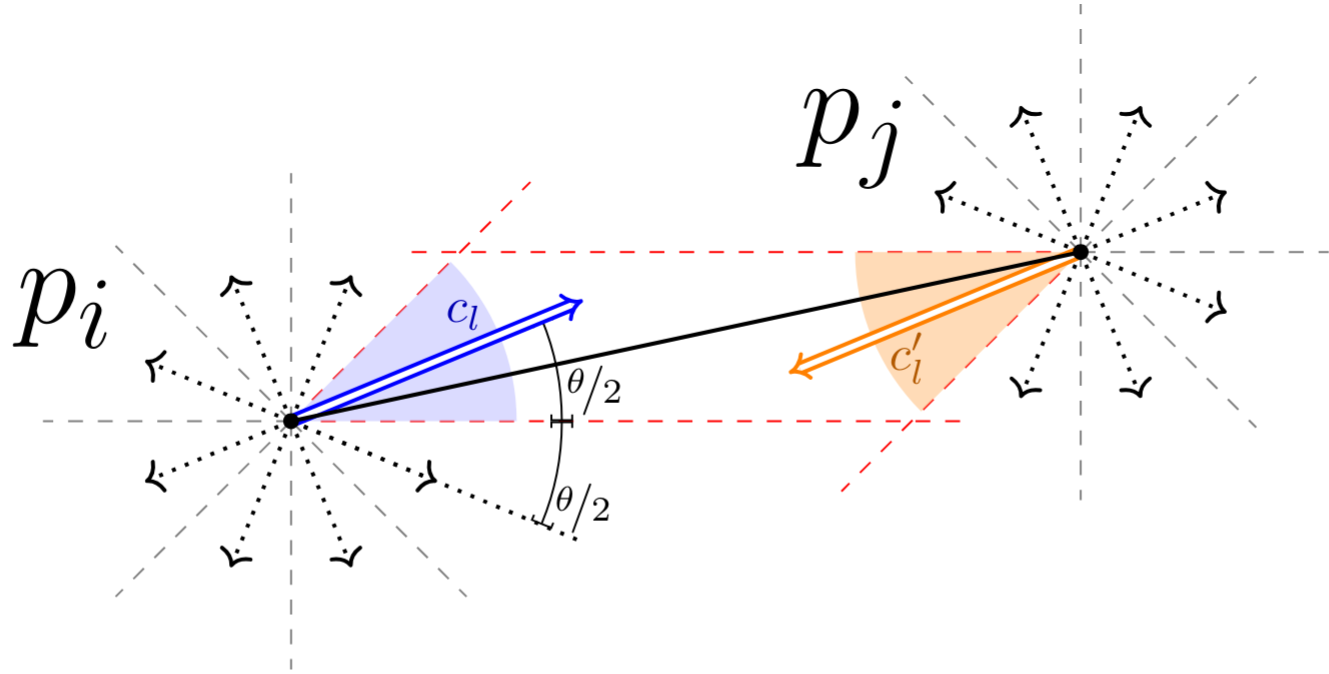
\includegraphics[height=5cm]{MSC/discrete.png}
    \end{minipage}
\end{frame}

\begin{frame}{}
    \begin{obs}
        Cada solução ótima de custo $\theta N$ corresponde a uma função \mbox{$\hat h\colon P \to [4M-1]^{N+1}$}.
    \end{obs}
\end{frame}

\begin{frame}{}
    \begin{obs}
        \label{obs:msc2d}
        Seja $t^*$ o ótimo de $\cali$. Então, $t^* \leq 3\pi\ceil{\log_2(k+1)}$
    \end{obs}
\end{frame}

\begin{frame}{}
    Pela \ref{obs:msc2d}ª Observação, existe uma solução de $\hat \cali$ com custo $\theta N$, onde:

    \bigskip
    \centering
    $N \leq \frac{3\pi\ceil{\log_2(k+1)}}{\theta} = 6\floor{\nicefrac{\pi}{\lambda}} \ceil{\log_2(k+1)}$
\end{frame}

\begin{frame}{}
    \centering
    Particionamos o intervalo de tempo $[0,\ (N+1) \theta)$:

    \pause
    \vspace*{2cm}
    \begin{minipage}{\linewidth}
        \centering
        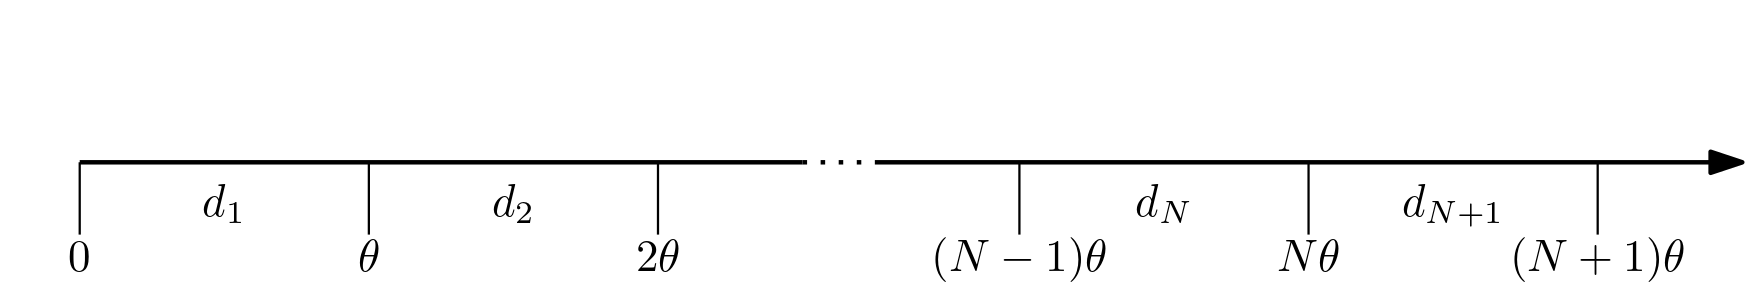
\includegraphics[width=10cm]{MSC/interval.png}
    \end{minipage}
\end{frame}

\begin{frame}{}
    \only<1>{\begin{lem}
        \label{lemma:1}
        Existe uma solução de custo no máximo $\floor{\nicefrac{t^*}{\theta}} \theta$ para $\hat \cali$, que mapeia arestas para pontos em $\{i\cdot \theta\ |\ i \in [N]\}$.
    \end{lem}}

    \centering 
    \only<2>{Seja {\color{blue} $\cals^*$} uma solução ótima para $\cali$.}
    \only<3>{Se o ângulo entre $\mathbf{e}$ e $\mathbf{f}$ não é zero, então ele é ao menos $\lambda>\theta$:}
    \only<4>{Caso contrário, o ângulo entre $\mathbf{e}$ e $\mathbf{f}$ é zero:}

    \begin{minipage}{\linewidth}
        \vspace*{2cm}
        \centering
        \only<3>{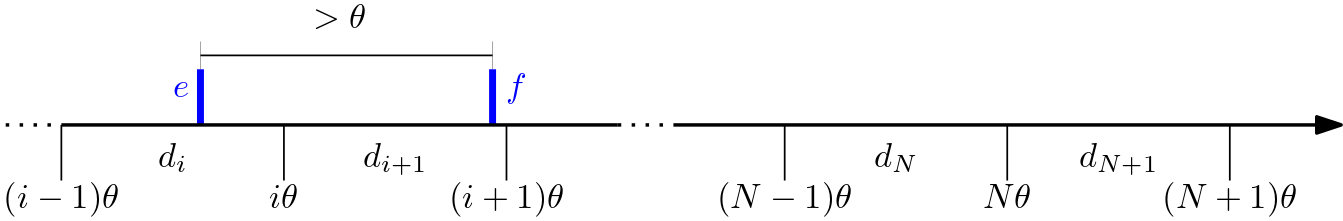
\includegraphics[width=10cm]{MSC/lemma/lema_1.png}}%
        \only<4>{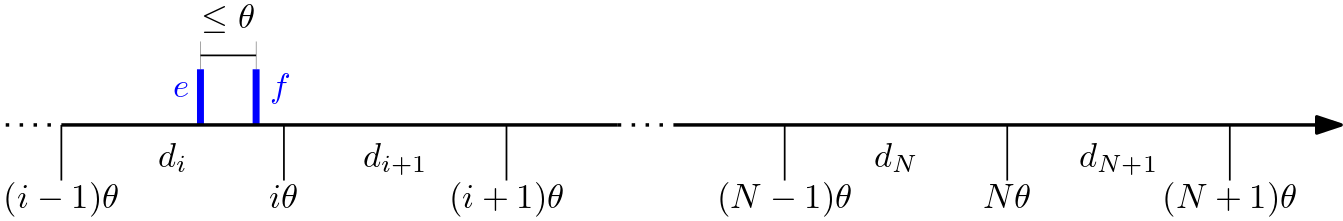
\includegraphics[width=10cm]{MSC/lemma/lema_2.png}}%
    \end{minipage}
\end{frame}

\begin{frame}{}
    \centering
    Construímos uma solução {\color{red} $\hat \cals$} para $\hat \cali$ a partir de {\color{blue} $\cals^*$}:

    \begin{minipage}{\linewidth}
        \vspace*{2cm}
        \centering
        \only<2>{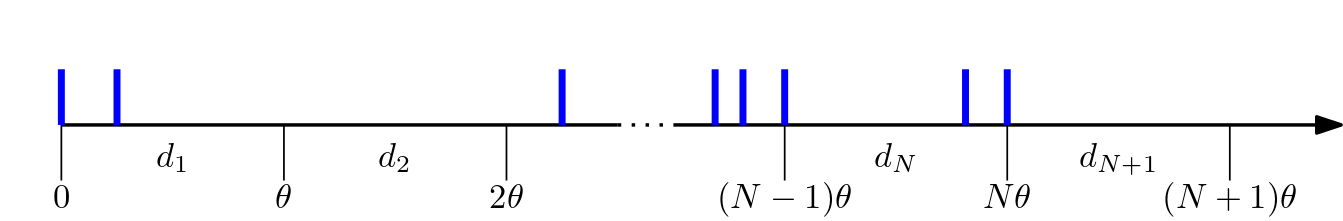
\includegraphics[width=10cm]{MSC/lemma/lema_3.png} \hfill{}\\\phantom{\qed}}%
        \only<3>{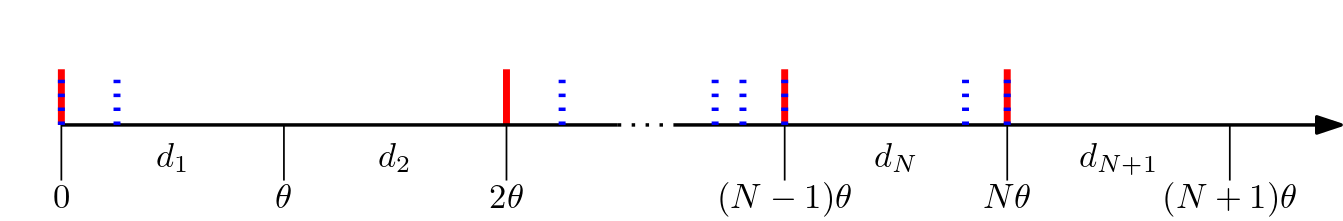
\includegraphics[width=10cm]{MSC/lemma/lema_4.png} \hfill{}\\\qed}%
    \end{minipage}
\end{frame}

\begin{frame}{}
    Usando programação dinâmica sobre a decomposição em árvore calculamos uma solução ótima $\hat \cals^*$ para $\hat\cali$ em tempo:

    \bigskip
    \centering
    $N^{O(k^2)}\cdot M^{O(Nk)}\cdot k^{O(1)} \cdot n = \lambda^{-O(k^2+\frac{k\log k}{\lambda})}\cdot (\log k)^{O(k^2)}\cdot n$
\end{frame}

\begin{frame}{}
    \centering
    \only<1>{Seja {\color{red} $\hat \cals^*$} uma solução ótima para $\hat \cali$:}
    \only<3>{Construímos uma solução {\color{blue} $\cals$} para $\cali$ a partir de {\color{red} $\hat \cals^*$}:}

    \only<2>{
        \begin{itemize}
            \item Se o ângulo entre $\mathbf{e}$ e $\mathbf{f}$ não é zero, então é maior que $\theta$;
            
            \item Logo, $|{\color{red} \hat \cals^*}(\mathbf{e})-{\color{red} \hat \cals^*}(\mathbf{f})|> \theta$, e não pertencem ao mesmo $E^i$.
        \end{itemize}
    }

    \begin{minipage}{\linewidth}
        \vspace*{2cm}
        \centering
        \only<1>{
\includegraphics[width=10cm]{MSC/final/final_1.png}}%
        \only<3>{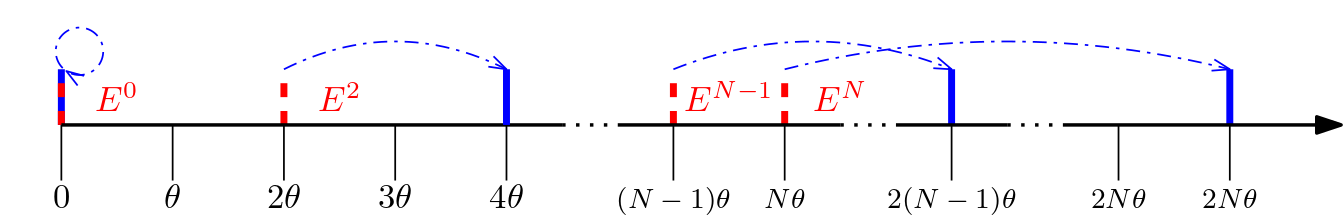
\includegraphics[width=10cm]{MSC/final/final_2.png}}%
    \end{minipage}
\end{frame}

\begin{frame}{}
    \centering
    \only<1,7>{Arestas no mesmo $E^i$ \checkmark}
    \only<2-6>{$\mathbf{e} \in H^i$ e $\mathbf{f} \in H^j$ onde $i\ne j$:\\\bigskip}
    \only<5>{\centering Sabemos que $|{\color{red} \hat \cals^*}(e) - {\color{red} \hat \cals^*}(f)|=|i-j|\cdot \theta \ge \phi$}
    \only<6>{\centering Logo, por definição, $|{\color{blue} \cals}(e) - {\color{blue} \cals}(f)| = 2|i-j| \cdot \theta \ge \phi + \theta$ e ${\color{blue} \cals}$ é válido}

    \only<7>{$\mathbf{e} \in H^i$ e $\mathbf{f} \in H^j$ onde $i\ne j$ \checkmark\\\bigskip}
    \only<7>{\centering Portanto, pelo \ref{lemma:1}º Lema, o custo é no máximo $2\floor{\nicefrac{t^*}{\theta}}\theta \le 2t^*$ \qed}

    \begin{minipage}{\linewidth}
        \vspace*{0.5cm}
        \centering
        \only<2>{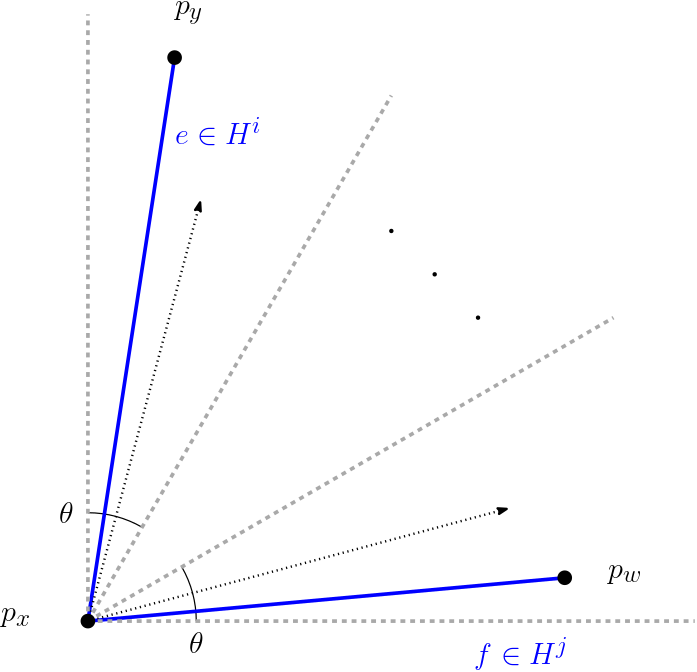
\includegraphics[height=6cm]{MSC/end/end_2.png}}%
        \only<3>{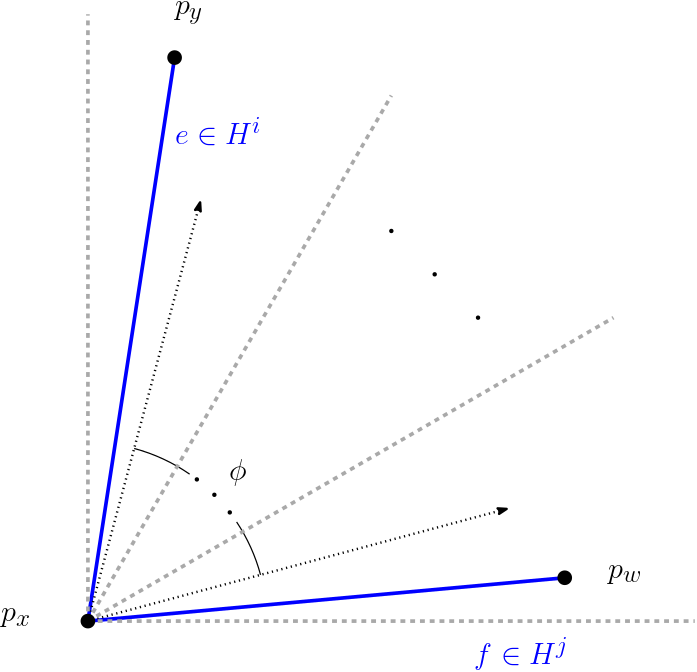
\includegraphics[height=6cm]{MSC/end/end_3.png}}%
        \only<4-6>{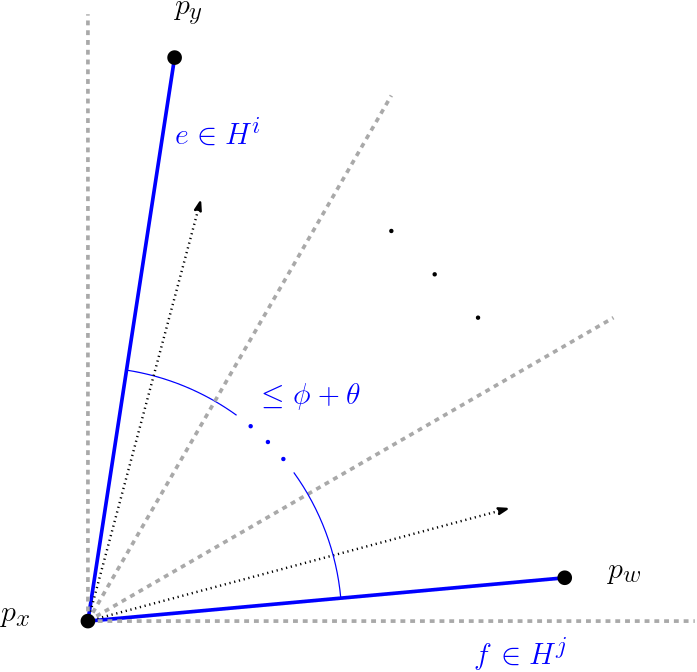
\includegraphics[height=6cm]{MSC/end/end_4.png}}%
    \end{minipage}
\end{frame}

\begin{frame}{Nosso Resultado}
  \setbeamercolor{block body}{bg=green!35!white}
  \begin{cor}
    Existe uma $5$-aproximação para o MSC em 2D em grafos planares parametrizada por $\lceil \nicefrac{1}{\lambda} \rceil$, que roda em tempo $\lambda^{-O(\nicefrac{1}{\lambda})} \cdot n + O(n^2)$.
  \end{cor}
\end{frame}


\section{Trabalhos Futuros}
\subseqslide

\begin{frame}{Freeze-Tag Problem}
  \begin{itemize}[<+->]

    \item NP-dificuldade do FTP para a distância $L_1$ no plano;

    \item Aproximação de fator constante para métricas gerais ou árvores;

    \begin{itemize}[<+->]
        \item O melhor fator conhecido é $O(\sqrt{\log n})$~\cite{Kne05}.
    \end{itemize}

    \item Combinação CP + PTAS com outros problemas NP-difíceis.

  \end{itemize}
\end{frame}

\begin{frame}{Angular Freeze-Tag Problem}
  \begin{itemize}[<+->]

    \item $E$ e/ou $k$ no expoente do tempo de execução das aproximações;

    \item Dificuldade do AFTP para minimização da energia total;

    \item Melhor aproximação ou limitante inferior para 3D.

  \end{itemize}
\end{frame}

\begin{frame}{Minimum Scan Cover}
  \begin{itemize}[<+->]

    \item Eliminar a dependência de $\lambda$, melhorar o fator para $1+\varepsilon$ ou obter um \FPT exato;

    \item Para 3D, fornecer algum limite inferior ou superior não trivial.

  \end{itemize}
\end{frame}


\begin{frame}
  \large{\centerline{Obrigado a todos pela atenção...}}
  \pause
  \Huge{\centerline{Fim}}
\end{frame}

%-----------------------[ Bibliography ]---------------------------------------%

\appendix

\setbeamertemplate{bibliography item}[text]
\begin{frame}[allowframebreaks]
  \frametitle{Referências}
  {
    \tiny
    \bibliographystyle{alpha}
    \bibliography{bibliography}
  }
\end{frame}

%-----------------------[ Backup ]---------------------------------------------%


\end{document}
